% !TEX TS-program = pgfSweave
\RequirePackage{atbegshi}
\documentclass{article}

%% $ R CMD pgfsweave pgfSweave-vignette-source.Rnw



% \VignetteIndexEntry{The pgfSweave Package}
% \VignetteDepends{pgfSweave}
% \VignetteDepends{tikzDevice}

\usepackage[nogin,noae]{Sweave}
\usepackage[x11names]{xcolor}
\usepackage{tikz}
\usetikzlibrary{positioning,shapes.geometric,arrows}

\usepackage[parfill]{parskip}
\usepackage{fancyvrb}
\usepackage[margin=1.1in]{geometry}
\usepackage[colorlinks]{hyperref}
\newcommand{\lang}{\textsf}
\newcommand{\code}{\texttt}
\newcommand{\pkg}{\textbf}
\newcommand{\ques}[1]{\vspace{.5cm}\noindent{\bf\large#1}\vspace{.2cm}}

\title{The \pkg{pgfSweave} Package}
\author{Cameron Bracken and Charlie Sharpsteen}


\newcommand{\hlnumber}[1]{\textcolor[rgb]{0.0823529411764706,0.0784313725490196,0.709803921568627}{#1}}%
\newcommand{\hlfunctioncall}[1]{\textcolor[rgb]{1,0,0}{#1}}%
\newcommand{\hlstring}[1]{\textcolor[rgb]{0.6,0.6,1}{#1}}%
\newcommand{\hlkeyword}[1]{\textcolor[rgb]{0,0,0}{\textbf{#1}}}%
\newcommand{\hlargument}[1]{\textcolor[rgb]{0.694117647058824,0.247058823529412,0.0196078431372549}{#1}}%
\newcommand{\hlcomment}[1]{\textcolor[rgb]{0.8,0.8,0.8}{#1}}%
\newcommand{\hlroxygencomment}[1]{\textcolor[rgb]{0,0.592156862745098,1}{#1}}%
\newcommand{\hlformalargs}[1]{\textcolor[rgb]{0.0705882352941176,0.713725490196078,0.0705882352941176}{#1}}%
\newcommand{\hleqformalargs}[1]{\textcolor[rgb]{0.0705882352941176,0.713725490196078,0.0705882352941176}{#1}}%
\newcommand{\hlassignement}[1]{\textcolor[rgb]{0.215686274509804,0.215686274509804,0.384313725490196}{\textbf{#1}}}%
\newcommand{\hlpackage}[1]{\textcolor[rgb]{0.588235294117647,0.713725490196078,0.145098039215686}{#1}}%
\newcommand{\hlslot}[1]{\textit{#1}}%
\newcommand{\hlsymbol}[1]{\textcolor[rgb]{0,0,0}{#1}}%
\newcommand{\hlprompt}[1]{\textcolor[rgb]{0,0,0}{#1}}%

\usepackage{color}%
 
\newsavebox{\hlnormalsizeboxclosebrace}%
\newsavebox{\hlnormalsizeboxopenbrace}%
\newsavebox{\hlnormalsizeboxbackslash}%
\newsavebox{\hlnormalsizeboxlessthan}%
\newsavebox{\hlnormalsizeboxgreaterthan}%
\newsavebox{\hlnormalsizeboxdollar}%
\newsavebox{\hlnormalsizeboxunderscore}%
\newsavebox{\hlnormalsizeboxand}%
\newsavebox{\hlnormalsizeboxhash}%
\newsavebox{\hlnormalsizeboxat}%
\newsavebox{\hlnormalsizeboxpercent}% 
\newsavebox{\hlnormalsizeboxhat}%
\newsavebox{\hlnormalsizeboxsinglequote}%
\newsavebox{\hlnormalsizeboxbacktick}%

\setbox\hlnormalsizeboxopenbrace=\hbox{\begin{normalsize}\verb.{.\end{normalsize}}%
\setbox\hlnormalsizeboxclosebrace=\hbox{\begin{normalsize}\verb.}.\end{normalsize}}%
\setbox\hlnormalsizeboxlessthan=\hbox{\begin{normalsize}\verb.<.\end{normalsize}}%
\setbox\hlnormalsizeboxdollar=\hbox{\begin{normalsize}\verb.$.\end{normalsize}}%
\setbox\hlnormalsizeboxunderscore=\hbox{\begin{normalsize}\verb._.\end{normalsize}}%
\setbox\hlnormalsizeboxand=\hbox{\begin{normalsize}\verb.&.\end{normalsize}}%
\setbox\hlnormalsizeboxhash=\hbox{\begin{normalsize}\verb.#.\end{normalsize}}%
\setbox\hlnormalsizeboxat=\hbox{\begin{normalsize}\verb.@.\end{normalsize}}%
\setbox\hlnormalsizeboxbackslash=\hbox{\begin{normalsize}\verb.\.\end{normalsize}}%
\setbox\hlnormalsizeboxgreaterthan=\hbox{\begin{normalsize}\verb.>.\end{normalsize}}%
\setbox\hlnormalsizeboxpercent=\hbox{\begin{normalsize}\verb.%.\end{normalsize}}%
\setbox\hlnormalsizeboxhat=\hbox{\begin{normalsize}\verb.^.\end{normalsize}}%
\setbox\hlnormalsizeboxsinglequote=\hbox{\begin{normalsize}\verb.'.\end{normalsize}}%
\setbox\hlnormalsizeboxbacktick=\hbox{\begin{normalsize}\verb.`.\end{normalsize}}%
\setbox\hlnormalsizeboxhat=\hbox{\begin{normalsize}\verb.^.\end{normalsize}}%



\newsavebox{\hltinyboxclosebrace}%
\newsavebox{\hltinyboxopenbrace}%
\newsavebox{\hltinyboxbackslash}%
\newsavebox{\hltinyboxlessthan}%
\newsavebox{\hltinyboxgreaterthan}%
\newsavebox{\hltinyboxdollar}%
\newsavebox{\hltinyboxunderscore}%
\newsavebox{\hltinyboxand}%
\newsavebox{\hltinyboxhash}%
\newsavebox{\hltinyboxat}%
\newsavebox{\hltinyboxpercent}% 
\newsavebox{\hltinyboxhat}%
\newsavebox{\hltinyboxsinglequote}%
\newsavebox{\hltinyboxbacktick}%

\setbox\hltinyboxopenbrace=\hbox{\begin{tiny}\verb.{.\end{tiny}}%
\setbox\hltinyboxclosebrace=\hbox{\begin{tiny}\verb.}.\end{tiny}}%
\setbox\hltinyboxlessthan=\hbox{\begin{tiny}\verb.<.\end{tiny}}%
\setbox\hltinyboxdollar=\hbox{\begin{tiny}\verb.$.\end{tiny}}%
\setbox\hltinyboxunderscore=\hbox{\begin{tiny}\verb._.\end{tiny}}%
\setbox\hltinyboxand=\hbox{\begin{tiny}\verb.&.\end{tiny}}%
\setbox\hltinyboxhash=\hbox{\begin{tiny}\verb.#.\end{tiny}}%
\setbox\hltinyboxat=\hbox{\begin{tiny}\verb.@.\end{tiny}}%
\setbox\hltinyboxbackslash=\hbox{\begin{tiny}\verb.\.\end{tiny}}%
\setbox\hltinyboxgreaterthan=\hbox{\begin{tiny}\verb.>.\end{tiny}}%
\setbox\hltinyboxpercent=\hbox{\begin{tiny}\verb.%.\end{tiny}}%
\setbox\hltinyboxhat=\hbox{\begin{tiny}\verb.^.\end{tiny}}%
\setbox\hltinyboxsinglequote=\hbox{\begin{tiny}\verb.'.\end{tiny}}%
\setbox\hltinyboxbacktick=\hbox{\begin{tiny}\verb.`.\end{tiny}}%
\setbox\hltinyboxhat=\hbox{\begin{tiny}\verb.^.\end{tiny}}%



\newsavebox{\hlscriptsizeboxclosebrace}%
\newsavebox{\hlscriptsizeboxopenbrace}%
\newsavebox{\hlscriptsizeboxbackslash}%
\newsavebox{\hlscriptsizeboxlessthan}%
\newsavebox{\hlscriptsizeboxgreaterthan}%
\newsavebox{\hlscriptsizeboxdollar}%
\newsavebox{\hlscriptsizeboxunderscore}%
\newsavebox{\hlscriptsizeboxand}%
\newsavebox{\hlscriptsizeboxhash}%
\newsavebox{\hlscriptsizeboxat}%
\newsavebox{\hlscriptsizeboxpercent}% 
\newsavebox{\hlscriptsizeboxhat}%
\newsavebox{\hlscriptsizeboxsinglequote}%
\newsavebox{\hlscriptsizeboxbacktick}%

\setbox\hlscriptsizeboxopenbrace=\hbox{\begin{scriptsize}\verb.{.\end{scriptsize}}%
\setbox\hlscriptsizeboxclosebrace=\hbox{\begin{scriptsize}\verb.}.\end{scriptsize}}%
\setbox\hlscriptsizeboxlessthan=\hbox{\begin{scriptsize}\verb.<.\end{scriptsize}}%
\setbox\hlscriptsizeboxdollar=\hbox{\begin{scriptsize}\verb.$.\end{scriptsize}}%
\setbox\hlscriptsizeboxunderscore=\hbox{\begin{scriptsize}\verb._.\end{scriptsize}}%
\setbox\hlscriptsizeboxand=\hbox{\begin{scriptsize}\verb.&.\end{scriptsize}}%
\setbox\hlscriptsizeboxhash=\hbox{\begin{scriptsize}\verb.#.\end{scriptsize}}%
\setbox\hlscriptsizeboxat=\hbox{\begin{scriptsize}\verb.@.\end{scriptsize}}%
\setbox\hlscriptsizeboxbackslash=\hbox{\begin{scriptsize}\verb.\.\end{scriptsize}}%
\setbox\hlscriptsizeboxgreaterthan=\hbox{\begin{scriptsize}\verb.>.\end{scriptsize}}%
\setbox\hlscriptsizeboxpercent=\hbox{\begin{scriptsize}\verb.%.\end{scriptsize}}%
\setbox\hlscriptsizeboxhat=\hbox{\begin{scriptsize}\verb.^.\end{scriptsize}}%
\setbox\hlscriptsizeboxsinglequote=\hbox{\begin{scriptsize}\verb.'.\end{scriptsize}}%
\setbox\hlscriptsizeboxbacktick=\hbox{\begin{scriptsize}\verb.`.\end{scriptsize}}%
\setbox\hlscriptsizeboxhat=\hbox{\begin{scriptsize}\verb.^.\end{scriptsize}}%



\newsavebox{\hlfootnotesizeboxclosebrace}%
\newsavebox{\hlfootnotesizeboxopenbrace}%
\newsavebox{\hlfootnotesizeboxbackslash}%
\newsavebox{\hlfootnotesizeboxlessthan}%
\newsavebox{\hlfootnotesizeboxgreaterthan}%
\newsavebox{\hlfootnotesizeboxdollar}%
\newsavebox{\hlfootnotesizeboxunderscore}%
\newsavebox{\hlfootnotesizeboxand}%
\newsavebox{\hlfootnotesizeboxhash}%
\newsavebox{\hlfootnotesizeboxat}%
\newsavebox{\hlfootnotesizeboxpercent}% 
\newsavebox{\hlfootnotesizeboxhat}%
\newsavebox{\hlfootnotesizeboxsinglequote}%
\newsavebox{\hlfootnotesizeboxbacktick}%

\setbox\hlfootnotesizeboxopenbrace=\hbox{\begin{footnotesize}\verb.{.\end{footnotesize}}%
\setbox\hlfootnotesizeboxclosebrace=\hbox{\begin{footnotesize}\verb.}.\end{footnotesize}}%
\setbox\hlfootnotesizeboxlessthan=\hbox{\begin{footnotesize}\verb.<.\end{footnotesize}}%
\setbox\hlfootnotesizeboxdollar=\hbox{\begin{footnotesize}\verb.$.\end{footnotesize}}%
\setbox\hlfootnotesizeboxunderscore=\hbox{\begin{footnotesize}\verb._.\end{footnotesize}}%
\setbox\hlfootnotesizeboxand=\hbox{\begin{footnotesize}\verb.&.\end{footnotesize}}%
\setbox\hlfootnotesizeboxhash=\hbox{\begin{footnotesize}\verb.#.\end{footnotesize}}%
\setbox\hlfootnotesizeboxat=\hbox{\begin{footnotesize}\verb.@.\end{footnotesize}}%
\setbox\hlfootnotesizeboxbackslash=\hbox{\begin{footnotesize}\verb.\.\end{footnotesize}}%
\setbox\hlfootnotesizeboxgreaterthan=\hbox{\begin{footnotesize}\verb.>.\end{footnotesize}}%
\setbox\hlfootnotesizeboxpercent=\hbox{\begin{footnotesize}\verb.%.\end{footnotesize}}%
\setbox\hlfootnotesizeboxhat=\hbox{\begin{footnotesize}\verb.^.\end{footnotesize}}%
\setbox\hlfootnotesizeboxsinglequote=\hbox{\begin{footnotesize}\verb.'.\end{footnotesize}}%
\setbox\hlfootnotesizeboxbacktick=\hbox{\begin{footnotesize}\verb.`.\end{footnotesize}}%
\setbox\hlfootnotesizeboxhat=\hbox{\begin{footnotesize}\verb.^.\end{footnotesize}}%



\newsavebox{\hlsmallboxclosebrace}%
\newsavebox{\hlsmallboxopenbrace}%
\newsavebox{\hlsmallboxbackslash}%
\newsavebox{\hlsmallboxlessthan}%
\newsavebox{\hlsmallboxgreaterthan}%
\newsavebox{\hlsmallboxdollar}%
\newsavebox{\hlsmallboxunderscore}%
\newsavebox{\hlsmallboxand}%
\newsavebox{\hlsmallboxhash}%
\newsavebox{\hlsmallboxat}%
\newsavebox{\hlsmallboxpercent}% 
\newsavebox{\hlsmallboxhat}%
\newsavebox{\hlsmallboxsinglequote}%
\newsavebox{\hlsmallboxbacktick}%

\setbox\hlsmallboxopenbrace=\hbox{\begin{small}\verb.{.\end{small}}%
\setbox\hlsmallboxclosebrace=\hbox{\begin{small}\verb.}.\end{small}}%
\setbox\hlsmallboxlessthan=\hbox{\begin{small}\verb.<.\end{small}}%
\setbox\hlsmallboxdollar=\hbox{\begin{small}\verb.$.\end{small}}%
\setbox\hlsmallboxunderscore=\hbox{\begin{small}\verb._.\end{small}}%
\setbox\hlsmallboxand=\hbox{\begin{small}\verb.&.\end{small}}%
\setbox\hlsmallboxhash=\hbox{\begin{small}\verb.#.\end{small}}%
\setbox\hlsmallboxat=\hbox{\begin{small}\verb.@.\end{small}}%
\setbox\hlsmallboxbackslash=\hbox{\begin{small}\verb.\.\end{small}}%
\setbox\hlsmallboxgreaterthan=\hbox{\begin{small}\verb.>.\end{small}}%
\setbox\hlsmallboxpercent=\hbox{\begin{small}\verb.%.\end{small}}%
\setbox\hlsmallboxhat=\hbox{\begin{small}\verb.^.\end{small}}%
\setbox\hlsmallboxsinglequote=\hbox{\begin{small}\verb.'.\end{small}}%
\setbox\hlsmallboxbacktick=\hbox{\begin{small}\verb.`.\end{small}}%
\setbox\hlsmallboxhat=\hbox{\begin{small}\verb.^.\end{small}}%



\newsavebox{\hllargeboxclosebrace}%
\newsavebox{\hllargeboxopenbrace}%
\newsavebox{\hllargeboxbackslash}%
\newsavebox{\hllargeboxlessthan}%
\newsavebox{\hllargeboxgreaterthan}%
\newsavebox{\hllargeboxdollar}%
\newsavebox{\hllargeboxunderscore}%
\newsavebox{\hllargeboxand}%
\newsavebox{\hllargeboxhash}%
\newsavebox{\hllargeboxat}%
\newsavebox{\hllargeboxpercent}% 
\newsavebox{\hllargeboxhat}%
\newsavebox{\hllargeboxsinglequote}%
\newsavebox{\hllargeboxbacktick}%

\setbox\hllargeboxopenbrace=\hbox{\begin{large}\verb.{.\end{large}}%
\setbox\hllargeboxclosebrace=\hbox{\begin{large}\verb.}.\end{large}}%
\setbox\hllargeboxlessthan=\hbox{\begin{large}\verb.<.\end{large}}%
\setbox\hllargeboxdollar=\hbox{\begin{large}\verb.$.\end{large}}%
\setbox\hllargeboxunderscore=\hbox{\begin{large}\verb._.\end{large}}%
\setbox\hllargeboxand=\hbox{\begin{large}\verb.&.\end{large}}%
\setbox\hllargeboxhash=\hbox{\begin{large}\verb.#.\end{large}}%
\setbox\hllargeboxat=\hbox{\begin{large}\verb.@.\end{large}}%
\setbox\hllargeboxbackslash=\hbox{\begin{large}\verb.\.\end{large}}%
\setbox\hllargeboxgreaterthan=\hbox{\begin{large}\verb.>.\end{large}}%
\setbox\hllargeboxpercent=\hbox{\begin{large}\verb.%.\end{large}}%
\setbox\hllargeboxhat=\hbox{\begin{large}\verb.^.\end{large}}%
\setbox\hllargeboxsinglequote=\hbox{\begin{large}\verb.'.\end{large}}%
\setbox\hllargeboxbacktick=\hbox{\begin{large}\verb.`.\end{large}}%
\setbox\hllargeboxhat=\hbox{\begin{large}\verb.^.\end{large}}%



\newsavebox{\hlLargeboxclosebrace}%
\newsavebox{\hlLargeboxopenbrace}%
\newsavebox{\hlLargeboxbackslash}%
\newsavebox{\hlLargeboxlessthan}%
\newsavebox{\hlLargeboxgreaterthan}%
\newsavebox{\hlLargeboxdollar}%
\newsavebox{\hlLargeboxunderscore}%
\newsavebox{\hlLargeboxand}%
\newsavebox{\hlLargeboxhash}%
\newsavebox{\hlLargeboxat}%
\newsavebox{\hlLargeboxpercent}% 
\newsavebox{\hlLargeboxhat}%
\newsavebox{\hlLargeboxsinglequote}%
\newsavebox{\hlLargeboxbacktick}%

\setbox\hlLargeboxopenbrace=\hbox{\begin{Large}\verb.{.\end{Large}}%
\setbox\hlLargeboxclosebrace=\hbox{\begin{Large}\verb.}.\end{Large}}%
\setbox\hlLargeboxlessthan=\hbox{\begin{Large}\verb.<.\end{Large}}%
\setbox\hlLargeboxdollar=\hbox{\begin{Large}\verb.$.\end{Large}}%
\setbox\hlLargeboxunderscore=\hbox{\begin{Large}\verb._.\end{Large}}%
\setbox\hlLargeboxand=\hbox{\begin{Large}\verb.&.\end{Large}}%
\setbox\hlLargeboxhash=\hbox{\begin{Large}\verb.#.\end{Large}}%
\setbox\hlLargeboxat=\hbox{\begin{Large}\verb.@.\end{Large}}%
\setbox\hlLargeboxbackslash=\hbox{\begin{Large}\verb.\.\end{Large}}%
\setbox\hlLargeboxgreaterthan=\hbox{\begin{Large}\verb.>.\end{Large}}%
\setbox\hlLargeboxpercent=\hbox{\begin{Large}\verb.%.\end{Large}}%
\setbox\hlLargeboxhat=\hbox{\begin{Large}\verb.^.\end{Large}}%
\setbox\hlLargeboxsinglequote=\hbox{\begin{Large}\verb.'.\end{Large}}%
\setbox\hlLargeboxbacktick=\hbox{\begin{Large}\verb.`.\end{Large}}%
\setbox\hlLargeboxhat=\hbox{\begin{Large}\verb.^.\end{Large}}%



\newsavebox{\hlLARGEboxclosebrace}%
\newsavebox{\hlLARGEboxopenbrace}%
\newsavebox{\hlLARGEboxbackslash}%
\newsavebox{\hlLARGEboxlessthan}%
\newsavebox{\hlLARGEboxgreaterthan}%
\newsavebox{\hlLARGEboxdollar}%
\newsavebox{\hlLARGEboxunderscore}%
\newsavebox{\hlLARGEboxand}%
\newsavebox{\hlLARGEboxhash}%
\newsavebox{\hlLARGEboxat}%
\newsavebox{\hlLARGEboxpercent}% 
\newsavebox{\hlLARGEboxhat}%
\newsavebox{\hlLARGEboxsinglequote}%
\newsavebox{\hlLARGEboxbacktick}%

\setbox\hlLARGEboxopenbrace=\hbox{\begin{LARGE}\verb.{.\end{LARGE}}%
\setbox\hlLARGEboxclosebrace=\hbox{\begin{LARGE}\verb.}.\end{LARGE}}%
\setbox\hlLARGEboxlessthan=\hbox{\begin{LARGE}\verb.<.\end{LARGE}}%
\setbox\hlLARGEboxdollar=\hbox{\begin{LARGE}\verb.$.\end{LARGE}}%
\setbox\hlLARGEboxunderscore=\hbox{\begin{LARGE}\verb._.\end{LARGE}}%
\setbox\hlLARGEboxand=\hbox{\begin{LARGE}\verb.&.\end{LARGE}}%
\setbox\hlLARGEboxhash=\hbox{\begin{LARGE}\verb.#.\end{LARGE}}%
\setbox\hlLARGEboxat=\hbox{\begin{LARGE}\verb.@.\end{LARGE}}%
\setbox\hlLARGEboxbackslash=\hbox{\begin{LARGE}\verb.\.\end{LARGE}}%
\setbox\hlLARGEboxgreaterthan=\hbox{\begin{LARGE}\verb.>.\end{LARGE}}%
\setbox\hlLARGEboxpercent=\hbox{\begin{LARGE}\verb.%.\end{LARGE}}%
\setbox\hlLARGEboxhat=\hbox{\begin{LARGE}\verb.^.\end{LARGE}}%
\setbox\hlLARGEboxsinglequote=\hbox{\begin{LARGE}\verb.'.\end{LARGE}}%
\setbox\hlLARGEboxbacktick=\hbox{\begin{LARGE}\verb.`.\end{LARGE}}%
\setbox\hlLARGEboxhat=\hbox{\begin{LARGE}\verb.^.\end{LARGE}}%



\newsavebox{\hlhugeboxclosebrace}%
\newsavebox{\hlhugeboxopenbrace}%
\newsavebox{\hlhugeboxbackslash}%
\newsavebox{\hlhugeboxlessthan}%
\newsavebox{\hlhugeboxgreaterthan}%
\newsavebox{\hlhugeboxdollar}%
\newsavebox{\hlhugeboxunderscore}%
\newsavebox{\hlhugeboxand}%
\newsavebox{\hlhugeboxhash}%
\newsavebox{\hlhugeboxat}%
\newsavebox{\hlhugeboxpercent}% 
\newsavebox{\hlhugeboxhat}%
\newsavebox{\hlhugeboxsinglequote}%
\newsavebox{\hlhugeboxbacktick}%

\setbox\hlhugeboxopenbrace=\hbox{\begin{huge}\verb.{.\end{huge}}%
\setbox\hlhugeboxclosebrace=\hbox{\begin{huge}\verb.}.\end{huge}}%
\setbox\hlhugeboxlessthan=\hbox{\begin{huge}\verb.<.\end{huge}}%
\setbox\hlhugeboxdollar=\hbox{\begin{huge}\verb.$.\end{huge}}%
\setbox\hlhugeboxunderscore=\hbox{\begin{huge}\verb._.\end{huge}}%
\setbox\hlhugeboxand=\hbox{\begin{huge}\verb.&.\end{huge}}%
\setbox\hlhugeboxhash=\hbox{\begin{huge}\verb.#.\end{huge}}%
\setbox\hlhugeboxat=\hbox{\begin{huge}\verb.@.\end{huge}}%
\setbox\hlhugeboxbackslash=\hbox{\begin{huge}\verb.\.\end{huge}}%
\setbox\hlhugeboxgreaterthan=\hbox{\begin{huge}\verb.>.\end{huge}}%
\setbox\hlhugeboxpercent=\hbox{\begin{huge}\verb.%.\end{huge}}%
\setbox\hlhugeboxhat=\hbox{\begin{huge}\verb.^.\end{huge}}%
\setbox\hlhugeboxsinglequote=\hbox{\begin{huge}\verb.'.\end{huge}}%
\setbox\hlhugeboxbacktick=\hbox{\begin{huge}\verb.`.\end{huge}}%
\setbox\hlhugeboxhat=\hbox{\begin{huge}\verb.^.\end{huge}}%



\newsavebox{\hlHugeboxclosebrace}%
\newsavebox{\hlHugeboxopenbrace}%
\newsavebox{\hlHugeboxbackslash}%
\newsavebox{\hlHugeboxlessthan}%
\newsavebox{\hlHugeboxgreaterthan}%
\newsavebox{\hlHugeboxdollar}%
\newsavebox{\hlHugeboxunderscore}%
\newsavebox{\hlHugeboxand}%
\newsavebox{\hlHugeboxhash}%
\newsavebox{\hlHugeboxat}%
\newsavebox{\hlHugeboxpercent}% 
\newsavebox{\hlHugeboxhat}%
\newsavebox{\hlHugeboxsinglequote}%
\newsavebox{\hlHugeboxbacktick}%

\setbox\hlHugeboxopenbrace=\hbox{\begin{Huge}\verb.{.\end{Huge}}%
\setbox\hlHugeboxclosebrace=\hbox{\begin{Huge}\verb.}.\end{Huge}}%
\setbox\hlHugeboxlessthan=\hbox{\begin{Huge}\verb.<.\end{Huge}}%
\setbox\hlHugeboxdollar=\hbox{\begin{Huge}\verb.$.\end{Huge}}%
\setbox\hlHugeboxunderscore=\hbox{\begin{Huge}\verb._.\end{Huge}}%
\setbox\hlHugeboxand=\hbox{\begin{Huge}\verb.&.\end{Huge}}%
\setbox\hlHugeboxhash=\hbox{\begin{Huge}\verb.#.\end{Huge}}%
\setbox\hlHugeboxat=\hbox{\begin{Huge}\verb.@.\end{Huge}}%
\setbox\hlHugeboxbackslash=\hbox{\begin{Huge}\verb.\.\end{Huge}}%
\setbox\hlHugeboxgreaterthan=\hbox{\begin{Huge}\verb.>.\end{Huge}}%
\setbox\hlHugeboxpercent=\hbox{\begin{Huge}\verb.%.\end{Huge}}%
\setbox\hlHugeboxhat=\hbox{\begin{Huge}\verb.^.\end{Huge}}%
\setbox\hlHugeboxsinglequote=\hbox{\begin{Huge}\verb.'.\end{Huge}}%
\setbox\hlHugeboxbacktick=\hbox{\begin{Huge}\verb.`.\end{Huge}}%
\setbox\hlHugeboxhat=\hbox{\begin{Huge}\verb.^.\end{Huge}}%
 

\def\urltilda{\kern -.15em\lower .7ex\hbox{\~{}}\kern .04em}%

\newcommand{\hlstd}[1]{\textcolor[rgb]{0,0,0}{#1}}%
\newcommand{\hlnum}[1]{\textcolor[rgb]{0.16,0.16,1}{#1}}
\newcommand{\hlesc}[1]{\textcolor[rgb]{1,0,1}{#1}}
\newcommand{\hlstr}[1]{\textcolor[rgb]{1,0,0}{#1}}
\newcommand{\hldstr}[1]{\textcolor[rgb]{0.51,0.51,0}{#1}}
\newcommand{\hlslc}[1]{\textcolor[rgb]{0.51,0.51,0.51}{\it{#1}}}
\newcommand{\hlcom}[1]{\textcolor[rgb]{0.51,0.51,0.51}{\it{#1}}}
\newcommand{\hldir}[1]{\textcolor[rgb]{0,0.51,0}{#1}}
\newcommand{\hlsym}[1]{\textcolor[rgb]{0,0,0}{#1}}
\newcommand{\hlline}[1]{\textcolor[rgb]{0.33,0.33,0.33}{#1}}
\newcommand{\hlkwa}[1]{\textcolor[rgb]{0,0,0}{\bf{#1}}}
\newcommand{\hlkwb}[1]{\textcolor[rgb]{0.51,0,0}{#1}}
\newcommand{\hlkwc}[1]{\textcolor[rgb]{0,0,0}{\bf{#1}}}
\newcommand{\hlkwd}[1]{\textcolor[rgb]{0,0,0.51}{#1}}

\begin{document}

%% Cache all of the code chunks and generate external figures by default 
%% the pgfSweave defaults are pdf=FALSE and eps=FALSE and pgf=FALSE and tikz=TRUE.
%% to get normal Sweave behavior set pgf=FALSE and external=FALSE 


\begin{center}
{\Large The \pkg{pgfSweave} Package}\\
{\large Cameron Bracken and Charlie Sharpsteen \\ \today}\vspace{1cm}
\end{center}

\tableofcontents

\clearpage
\section{Introduction} 
The \pkg{pgfSweave} package is about {\color{SteelBlue1}speed} and {\color{Sienna1}style}.  For {\color{SteelBlue1}speed}, the package provides capabilities for ``caching'' graphics generated with \pkg{Sweave} on top of the caching funcitonality of \pkg{cacheSweave}\footnote{\url{http://cran.r-project.org/web/packages/cacheSweave/index.html}}.  For {\color{Sienna1}style} the \pkg{pgfSweave} package facilitates the integration of \lang{R} graphics with \LaTeX\ reports through the \pkg{tikzDevice}\footnote{\url{http://cran.r-project.org/web/packages/tikzDevice/index.html}} package or the \pkg{eps2pgf}\footnote{\url{http://sourceforge.net/projects/eps2pgf/}} utility.  With these tools, figure labels are converted to \LaTeX{} strings so they match the style of the document and the full range of \LaTeX{} math symbols/equations are available.  In addition \pkg{pgfSweave} can produce syntax highlighted and/or cleaned up source code. 

The backbone of \pkg{pgfSweave} is a a new driver for \pkg{Sweave} (\code
{pgfSweaveDriver}). The driver provides new chunk options \code{tikz}, \code{pgf} and \code
{external}, \code{sanitize}, \code{highlight} and \code{tidy} on top of the \code{cache} option provided by \pkg{cacheSweave}.  This package 
started as a fork of \pkg{cacheSweave}. This document highlights the features and usage of 
\pkg{pgfSweave}.  This document assumes familiarity with \pkg{Sweave}.  

%%%%%%%%%%%%%%%%%%%%%%%%%%%%%%%%%%%%%%%%%%%%%%%
%%%%%%%%%%%%%%%%%%%%%%%%%%%%%%%%%%%%%%%%%%%%%%%
\section{Motivation and Background} 

\pkg{Sweave} is a tool for generating ``reproducible research'' documents by embedding \lang{R} or \lang{S} ``code chunks'' directly into a \LaTeX{} document.  For small projects, this approach works well.  For large papers or projects, heavy data analysis or computation can cause document compilation times that are unacceptable.  The problem of performing lengthy computations in Sweave documents is not a new one.  Previous attempts to tackle this problem include the \pkg{cacheSweave} and \pkg{weaver}\footnote{\url{http://www.bioconductor.org/packages/2.3/bioc/html/weaver.html}} packages.  These packages address the problem that code chunks with lengthy computations are executed every time a document is compiled.  Both packages provide a \code{cache} option which saves R objects for quick access during successive compilations. The \pkg{cacheSweave} package stores results in a \pkg{filehash}\footnote{\url{http://cran.r-project.org/package=filehash}} databases while the \pkg{weaver} package stores RData files.  The benefit of the \pkg{cacheSweave} method is lazy loading of objects.  Both methods provide significant speedup for most \pkg{Sweave} documents, namely those which create objects in the global environment.

The existing methods have some drawbacks:

\begin{enumerate} 
\item Plots are not cached (since plots do not generally create objects in the global environment). If a plot takes a long time to generate, the same problem exists as when lengthy computations are present.  Ideally we would like to reuse a plot if the code that generated it has not changed. 
\item Consistency in style (font, point size) in automatically generated graphics is difficult to achieve.  The default font and point size in \lang{R} does not match \LaTeX{} very well and getting this to match precisely is tricky business.  The previously mentioned tools, \pkg{tikzDevice} and \pkg{eps2pgf}, counter this but using them with \pkg{Sweave} manually can be cumbersome.
\end{enumerate}

The \pkg{pgfSweave} package addresses these drawbacks.  The so called ``caching'' of plots is achieved with the help of three tools: the \TeX{} package \pkg{PGF}\footnote{\url{http://sourceforge.net/projects/pgf/}}  and either the command line utility \pkg{eps2pgf} or the \lang{R} package \pkg{tikzDevice}.  When we refer to the ``caching'' of a graphic we mean that if the code chunk which generated the graphic is unchanged, an image included from a file rather than regenerated from the code.  The \TeX{} package \pkg{pgf} provides the ability to ``externalize graphics.''  The effect of externalization is that graphics get extracted and compiled separately, saving time on subsequent compilations.  The externalization chapter in the \pkg {PGF/Ti\textit{k}Z} manual is extremely well written, and we refer the interested user there for more information.  Externalization plus some clever checking on the part of \pkg{pgfSweave} makes up the caching mechanism.  

The plot style consistency drawback is addressed by the handy options \code{tikz} and \code
{pgf} which allow for graphics to be output in these formats. Again, it is possible to do this 
manually but the chunk options make things easier. 


%%%%%%%%%%%%%%%%%%%%%%%%%%%%%%%%%%%%%%%%%%%%%%%%
%%%%%%%%%%%%%%%%%%%%%%%%%%%%%%%%%%%%%%%%%%%%%%%%
\section{System Requirements}
In general \pkg{pgfSweave} depends on:
\begin{enumerate}
\item A working \TeX{} distribution (such as TeXLive for linux and mac and MiKTex for Windows)
\item The java command line interpreter (i.e. the \code{java} command).  This is standard on most systems and is free to download otherwise. 
\item At least version 2.00 of the \pkg{PGF/Ti\textit{k}Z} package for \LaTeX{}. 
\end{enumerate}

That should be it for any *nix or Mac OS X system. 

\subsection{Windows specific requirements}

The \pkg{pgfSweave} package can work on Windows with some special care.  First of all it is strongly recommended that R be installed in a location that does not have spaces in its path name such as \texttt{C:$\backslash$R}.  This will save much grief when using \pkg{Sweave}. In addition, do the following in the order listed. 

\begin{enumerate}
\item Install Java. 
\item Install MiK\TeX{}. 
\item Upgrade to or install PGF 2.0 if not already done. 
\item Install Rtools\footnote{\url{http://www.murdoch-sutherland.com/Rtools/}}. Make sure to allow the Rtools installer to modify your PATH.  
\end{enumerate}

If everything is set up correctly, the commands \code{java} and \code{pdflatex} or \code{latex} should be available at the command prompt.    



%%%%%%%%%%%%%%%%%%%%%%%%%%%%%%%%%%%%%%%%%%%%%%%%
%%%%%%%%%%%%%%%%%%%%%%%%%%%%%%%%%%%%%%%%%%%%%%%%
\section{Usage}

We assume a familiarity with the usage of \pkg{Sweave}, for more information see the \pkg{Sweave} manual.\footnote{\url{http://www.stat.uni-muenchen.de/~leisch/Sweave/Sweave-manual.pdf}}  This section will explain the usage of the \code{tikz}, \code{pgf} and \code{external} options and then provide a complete example.

\subsection{The \code{tikz} option}
The first new code chunk option, \code{tikz}, acts the same as the \code{pdf} or \code{eps} options but instead of resulting in an \code{$\backslash$includegraphics\{\}} statement the 
result is an \code{$\backslash$input\{\}} statement. Consider the following code:

\begin{minipage}[!ht]{.5\linewidth}
Input:
\begin{Verbatim}[frame=single]
 \begin{figure}[ht]
 <<tikz-option,fig=T,tikz=T,echo=F>>=
     x <- rnorm(100)
     plot(x)
 @  
 \caption{caption}
 \label{fig:tikz-option}
 \end{figure}
\end{Verbatim}
\end{minipage}
\begin{minipage}[!ht]{.5\linewidth}
Output:
\begin{Verbatim}[frame=single]
 \begin{figure}[ht]
 \input{tikz-option.tikz}
 \caption{caption}
 \label{fig:tikz-option}
 \end{figure}
\end{Verbatim}
\end{minipage}

\vspace{.5cm}
The \code{.tikz} file is generated with the \pkg{tikzDevice} package.  {\color{red} This is the default graphics output for \pkg{pgfSweave}, the \code{tikz} option is set to \code{TRUE} by default.}

\subsection{The \code{pgf} option}
The second new code chunk option \code{pgf}, acts the same as the tikz option in that the result is an \code{$\backslash$input\{\}} statement.  Consider the following code:

\begin{minipage}[!ht]{.5\linewidth}
Input:
\begin{Verbatim}[frame=single]
 \begin{figure}[ht]
 <<pgf-option,fig=T,pgf=T,tikz=F,echo=F>>=
     x <- rnorm(100)
     plot(x)
 @  
 \caption{caption}
 \label{fig:pgf-option}
 \end{figure}
\end{Verbatim}
\end{minipage}
\begin{minipage}[!ht]{.5\linewidth}
Output:
\begin{Verbatim}[frame=single]
 \begin{figure}[ht]
 \input{pgf-option.pgf}
 \caption{caption}
 \label{fig:pgf-option}
 \end{figure}
\end{Verbatim}
\end{minipage}

\vspace{.5cm}

The \code{.pgf} file is generated with the \pkg{eps2pgf} utility. The \code{postscript} graphics device is used first to generate a \code{.eps} file.  Then the command \begin{verbatim}$ java -jar /path/to/eps2pgf.jar -m directcopy graphic.eps\end{verbatim} is run on every code chunk that has \code{fig=TRUE} and \code{pgf=TRUE}.  We do not  recommend using this option in favor of the \code{tikz} option.  Using the \code{pgf} option  involves two creation steps instead of one and it strips the \lang{R} text styles (such as boldface).

\subsection{The \code{sanitize} option}

This option is a boolean value that accesses the \code{tikz()} option of the same name.  Please see the \code{tikz()} documentation for more details. 

\subsection{The \code{external} option}

The external option is the interface to the graphics caching mechanism in \pkg{pgfSweave}. This option will wrap your graphics output in \code{$\backslash$beginpgfgraphicnamed} and \code{$\backslash$endpgfgraphicnamed}.

\begin{minipage}[!ht]{.55\linewidth}
Input:
\begin{Verbatim}[frame=single]
 \begin{figure}[ht]
 <<external,fig=T,tikz=T,external=T,echo=F>>=
     x <- rnorm(100)
     plot(x)
 @  
 \caption{caption}
 \label{fig:external-option}
 \end{figure}
\end{Verbatim}
\end{minipage}
\begin{minipage}[!ht]{.45\linewidth}
Output:
\begin{Verbatim}[frame=single]
 \begin{figure}[ht]
 \beginpgfgraphicnamed{external}
 \input{external.tikz}
 \endpgfgraphicnamed
 \caption{caption}
 \label{fig:external}
 \end{figure}
\end{Verbatim}
\end{minipage}

 When a graphic is newly created or when it has changed, \pkg{pgfSweave} will generate a command for externalizing that graphic in the shell script \code{$<$filename$>$.sh}.  This follows the process outlined in the externalization section of the pgf manual.  After the \pkg{Sweave} process is done the externalization commands are run.  This will create separate image files for each graphic. On later compilations this image file will simply be included instead of being regenerated.  
 

\subsection{The \code{$\backslash$pgfrealjobname} commmand}

Those familiar with the externalization mechanism in pgf will know that a command of the form \code{$\backslash$pgfrealjobname\{$<$basefilename$>$\}} in the header of your document is required when using externalization.   For example if you document is \code{main.Rnw} then your header should contain the line \code{$\backslash$pgfrealjobname\{main\}}. \pkg{pgfSweave} version 1.1 or later will add this for you automatically, so {\color{red} don't add it yourself!}.  This way if you rename your document, everything will still work out fine.  If you do add that line, \pkg{pgfSweave} will not add its own line.  
 
\subsection{The \code{tex.driver} option (Externalization Driver)}
The option \code{tex.driver} controls which engine (\code{latex}, \code{pdflatex}, \code{xelatex}, etc.) is used to externalize graphics.  The value of this option gets passed to the command created in the shell script that is written. For example if the value is \code{pdflatex} then only one command to externalize the graphic gets created in the shell script. For an external figure named ``figure-name'':

\begin{Verbatim}
    pdflatex --jobname=figure-name document-name.tex
\end{Verbatim}

If the value is \code{latex} then some extra commands are issues to convert dvi output to an eps file. For an external figure named ``figure-name'':

\begin{Verbatim}
    latex --jobname=figure-name document-name.tex
    dvipdf figure-name.dvi
    pdftops -eps document-name.pdf
\end{Verbatim}

The command \code{dvipdf} should come with any latex installation. The command \code{pdftops} is part of xpdf but should come with most latex distributions (it does not come with MacTeX for example).

\subsection{The \code{highlight} option}
Version 1.1.0 of \pkg{pgfSweave} introduced the \code{highlight} option.  The default is \code{TRUE} by default so code will be syntax-highlighted with the \pkg{highlight} package. To disable highlighting add \code{\textbackslash SweaveOpts\{highlight=F\}} to disable it. This option can be combined with the \code{keep.source} option or the \code{tidy} option.  For example:

The original code in the chunk looks like:

\begin{Verbatim}
        # here is a comment
    x <- numeric(100)
    for( i in 1:100){
        x[i] <- rnorm(1)
    }
        # OR
    y <- rnorm(100)
    
    plot(x,y)
\end{Verbatim}

Normal:
\begin{Schunk}
\begin{Sinput}
> x <- numeric(100)
> for (i in 1:100) {
+     x[i] <- rnorm(1)
+ }
> y <- rnorm(100)
> plot(x, y)
\end{Sinput}
\end{Schunk}


With Highlighting:
\hspace*{\fill}\\
\hlstd{}\ttfamily\noindent
\hlprompt{\usebox{\hlnormalsizeboxgreaterthan}{\ }}\hlsymbol{x}{\ }\hlassignement{\usebox{\hlnormalsizeboxlessthan}-}{\ }\hlfunctioncall{numeric}\hlkeyword{(}\hlnumber{100}\hlkeyword{)}\mbox{}
\normalfont
\hspace*{\fill}\\
\hlstd{}\ttfamily\noindent
\hlprompt{\usebox{\hlnormalsizeboxgreaterthan}{\ }}\hlkeyword{for}{\ }\hlkeyword{(}\hlsymbol{i}{\ }\hlkeyword{in}{\ }\hlnumber{1}\hlkeyword{:}\hlnumber{100}\hlkeyword{)}{\ }\hlkeyword{\usebox{\hlnormalsizeboxopenbrace}}\hspace*{\fill}\\
\hlstd{}\hlprompt{+{\ }}{\ }{\ }{\ }{\ }\hlsymbol{x}\hlkeyword{[}\hlsymbol{i}\hlkeyword{]}{\ }\hlassignement{\usebox{\hlnormalsizeboxlessthan}-}{\ }\hlfunctioncall{rnorm}\hlkeyword{(}\hlnumber{1}\hlkeyword{)}\hspace*{\fill}\\
\hlstd{}\hlprompt{+{\ }}\hlkeyword{\usebox{\hlnormalsizeboxclosebrace}}\mbox{}
\normalfont
\hspace*{\fill}\\
\hlstd{}\ttfamily\noindent
\hlprompt{\usebox{\hlnormalsizeboxgreaterthan}{\ }}\hlsymbol{y}{\ }\hlassignement{\usebox{\hlnormalsizeboxlessthan}-}{\ }\hlfunctioncall{rnorm}\hlkeyword{(}\hlnumber{100}\hlkeyword{)}\mbox{}
\normalfont
\hspace*{\fill}\\
\hlstd{}\ttfamily\noindent
\hlprompt{\usebox{\hlnormalsizeboxgreaterthan}{\ }}\hlfunctioncall{plot}\hlkeyword{(}\hlsymbol{x}\hlkeyword{,}{\ }\hlsymbol{y}\hlkeyword{)}\mbox{}
\normalfont
\hspace*{\fill}\\
\hlstd{}


\subsection{The \code{tidy} option}
Version 1.1.0 of \pkg{pgfSweave} introduced the \code{tidy} option.  This functionality was built into earlier releases, but is now available as an option for greater control.  Setting this chunk option to \code{TRUE} will clean up your code with the \code{tidy.source} function from the \code{animation} package. Using this option will not only preserve comments in the code but will reformat it's appearance.  This option takes precedent over the \code{keep.source} function but can be combined with the \code{highlight} option. Using the previous example:

Normal:
\begin{Schunk}
\begin{Sinput}
> x <- numeric(100)
> for (i in 1:100) {
+     x[i] <- rnorm(1)
+ }
> y <- rnorm(100)
> plot(x, y)
\end{Sinput}
\end{Schunk}


With Tidying:
\begin{Schunk}
\begin{Sinput}
>   # here is a comment
> x <- numeric(100)
> for (i in 1:100) {
+     x[i] <- rnorm(1)
+ }
>   # OR
> y <- rnorm(100)
> 
> plot(x, y)
\end{Sinput}
\end{Schunk}


With Tidying and Highlighting:
\hspace*{\fill}\\
\hlstd{}\ttfamily\noindent
\hlprompt{\usebox{\hlnormalsizeboxgreaterthan}{\ }}{\ }{\ }\hlcomment{\usebox{\hlnormalsizeboxhash}{\ }here{\ }is{\ }a{\ }comment}\mbox{}
\normalfont
\hspace*{\fill}\\
\hlstd{}\ttfamily\noindent
\hlprompt{\usebox{\hlnormalsizeboxgreaterthan}{\ }}\hlsymbol{x}{\ }\hlassignement{\usebox{\hlnormalsizeboxlessthan}-}{\ }\hlfunctioncall{numeric}\hlkeyword{(}\hlnumber{100}\hlkeyword{)}\mbox{}
\normalfont
\hspace*{\fill}\\
\hlstd{}\ttfamily\noindent
\hlprompt{\usebox{\hlnormalsizeboxgreaterthan}{\ }}\hlkeyword{for}{\ }\hlkeyword{(}\hlsymbol{i}{\ }\hlkeyword{in}{\ }\hlnumber{1}\hlkeyword{:}\hlnumber{100}\hlkeyword{)}{\ }\hlkeyword{\usebox{\hlnormalsizeboxopenbrace}}\hspace*{\fill}\\
\hlstd{}\hlprompt{+{\ }}{\ }{\ }{\ }{\ }\hlsymbol{x}\hlkeyword{[}\hlsymbol{i}\hlkeyword{]}{\ }\hlassignement{\usebox{\hlnormalsizeboxlessthan}-}{\ }\hlfunctioncall{rnorm}\hlkeyword{(}\hlnumber{1}\hlkeyword{)}\hspace*{\fill}\\
\hlstd{}\hlprompt{+{\ }}\hlkeyword{\usebox{\hlnormalsizeboxclosebrace}}\mbox{}
\normalfont
\hspace*{\fill}\\
\hlstd{}\ttfamily\noindent
\hlprompt{\usebox{\hlnormalsizeboxgreaterthan}{\ }}{\ }{\ }\hlcomment{\usebox{\hlnormalsizeboxhash}{\ }OR}\mbox{}
\normalfont
\hspace*{\fill}\\
\hlstd{}\ttfamily\noindent
\hlprompt{\usebox{\hlnormalsizeboxgreaterthan}{\ }}\hlsymbol{y}{\ }\hlassignement{\usebox{\hlnormalsizeboxlessthan}-}{\ }\hlfunctioncall{rnorm}\hlkeyword{(}\hlnumber{100}\hlkeyword{)}\mbox{}
\normalfont
\hspace*{\fill}\\
\hlstd{}\usebox{\hlnormalsizeboxgreaterthan}{\ }
\hspace*{\fill}\\
\hlstd{}\ttfamily\noindent
\hlprompt{\usebox{\hlnormalsizeboxgreaterthan}{\ }}\hlfunctioncall{plot}\hlkeyword{(}\hlsymbol{x}\hlkeyword{,}{\ }\hlsymbol{y}\hlkeyword{)}\mbox{}
\normalfont
\hspace*{\fill}\\
\hlstd{}


\subsection{Compilation Time}
The combination of \pkg{cacheSweave} code caching and \pkg{pgfSweave} figure caching can provide drastic decrease in compilation time.  The time speedup is highly dependednt on what code you are executing but using \pkg{pgfSweave} effectivly reduces the compilation time of \pkg{Sweave} to the time it takes to compile the \LaTeX{} document. 

\subsection{A Complete Example}
At this point we will provide a complete example.  The example from the \pkg{Sweave} manual is used to highlight the differences. The two frame below show the input Sweave file \texttt{pgfSweave-example-Rnw.in} and the resulting tex file \texttt{pgfSweave-example-tex.in}.

\VerbatimInput[frame=single,label={pgfSweave-example{}.Rnw},labelposition=all]{pgfSweave-example-Rnw.in}

On the input file run:
\begin{Verbatim}
R> library(pgfSweave)
R> pgfSweave('example.Rnw',pdf=T)
\end{Verbatim}

or 

\begin{Verbatim}
$ R CMD pgfsweave example.Rnw
\end{Verbatim}

And we get (from compiling \texttt{pgfSweave-example-tex.in}):

%\VerbatimInput[frame=single,label={pgfSweave-example{}.tex},labelposition=all]{pgfSweave-example-tex.in}

\begin{figure}[!hp]
\framebox{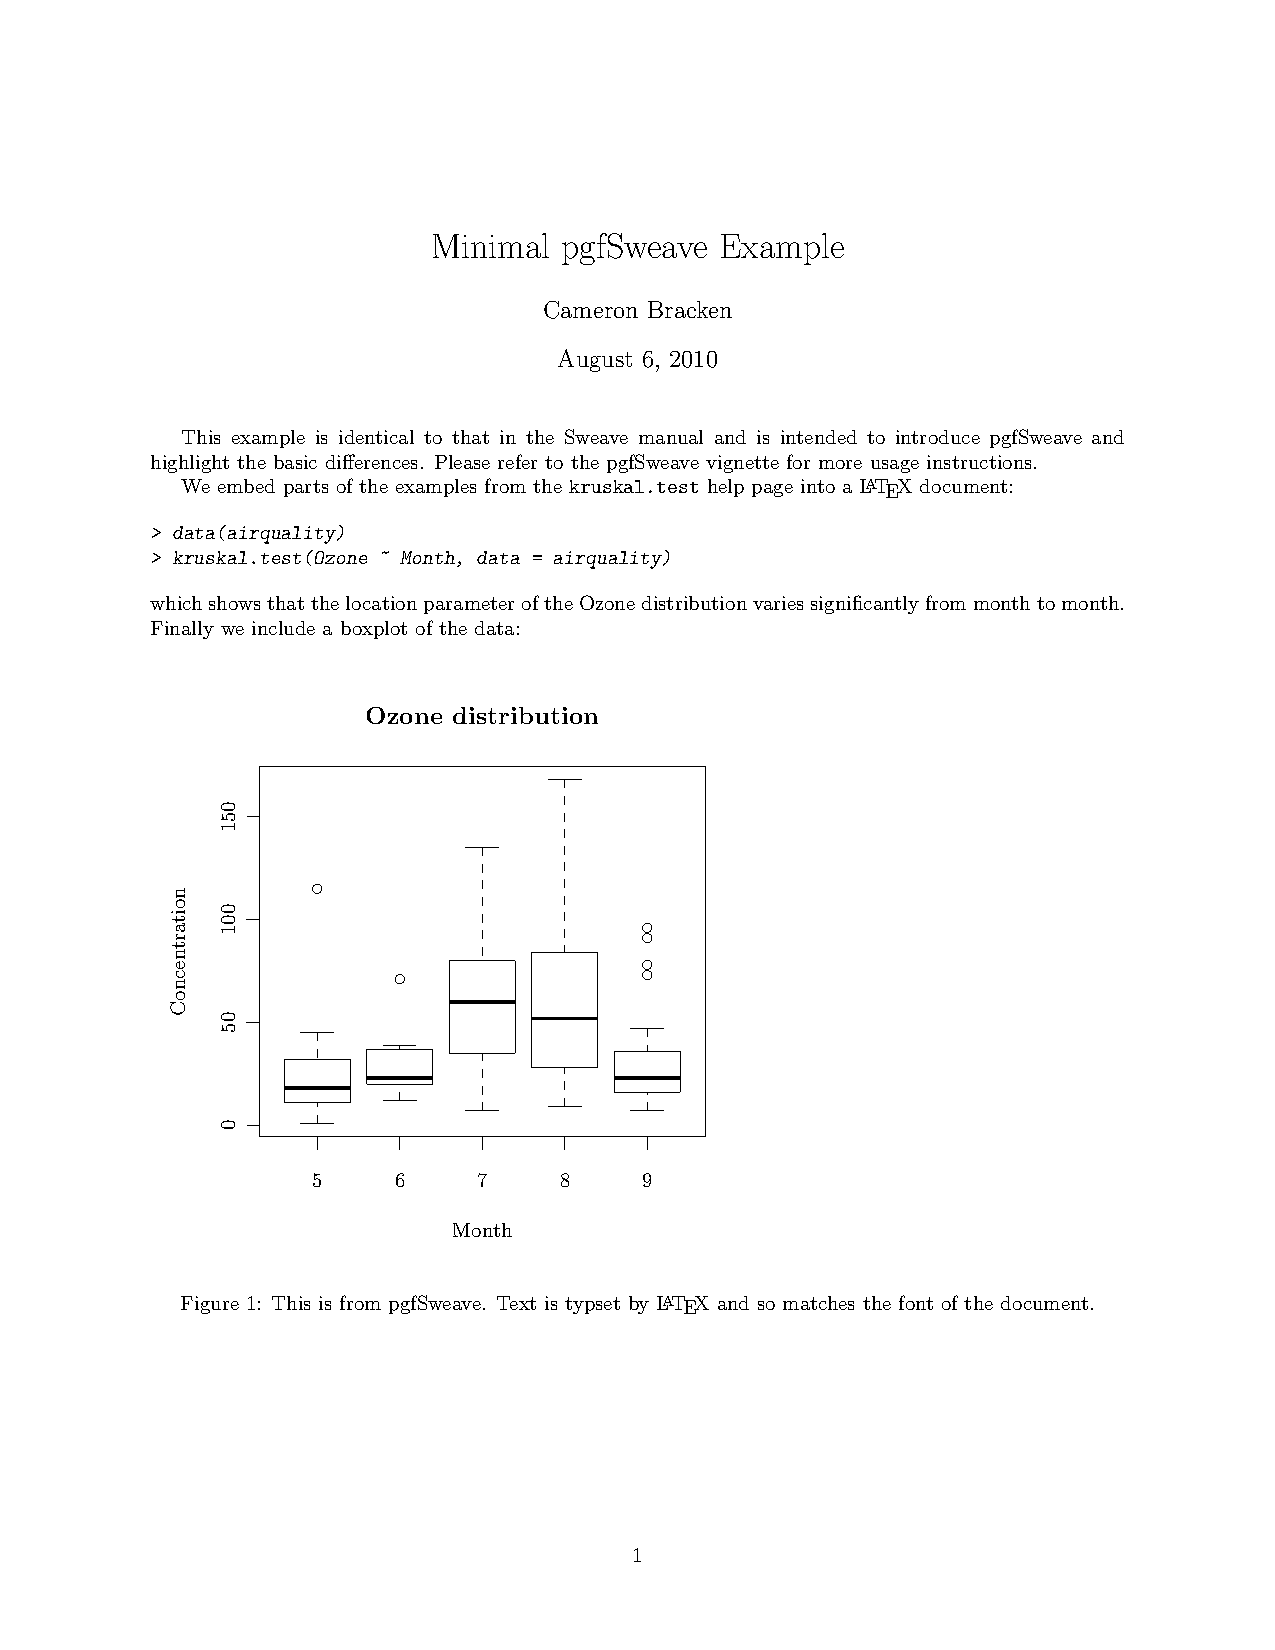
\includegraphics[width=\textwidth]{pgfSweave-example.pdf}}
\end{figure}

\clearpage

%%%%%%%%%%%%%%%%%%%%%%%%%%%%%%%%%%%%%%%%%%%%%%%%
%%%%%%%%%%%%%%%%%%%%%%%%%%%%%%%%%%%%%%%%%%%%%%%%
\section{The Process}
The process that \pkg{pgfSweave} uses when caching and externalization are turned on is outlined in the flow chart below:

\begin{figure}[!ht]
\centering
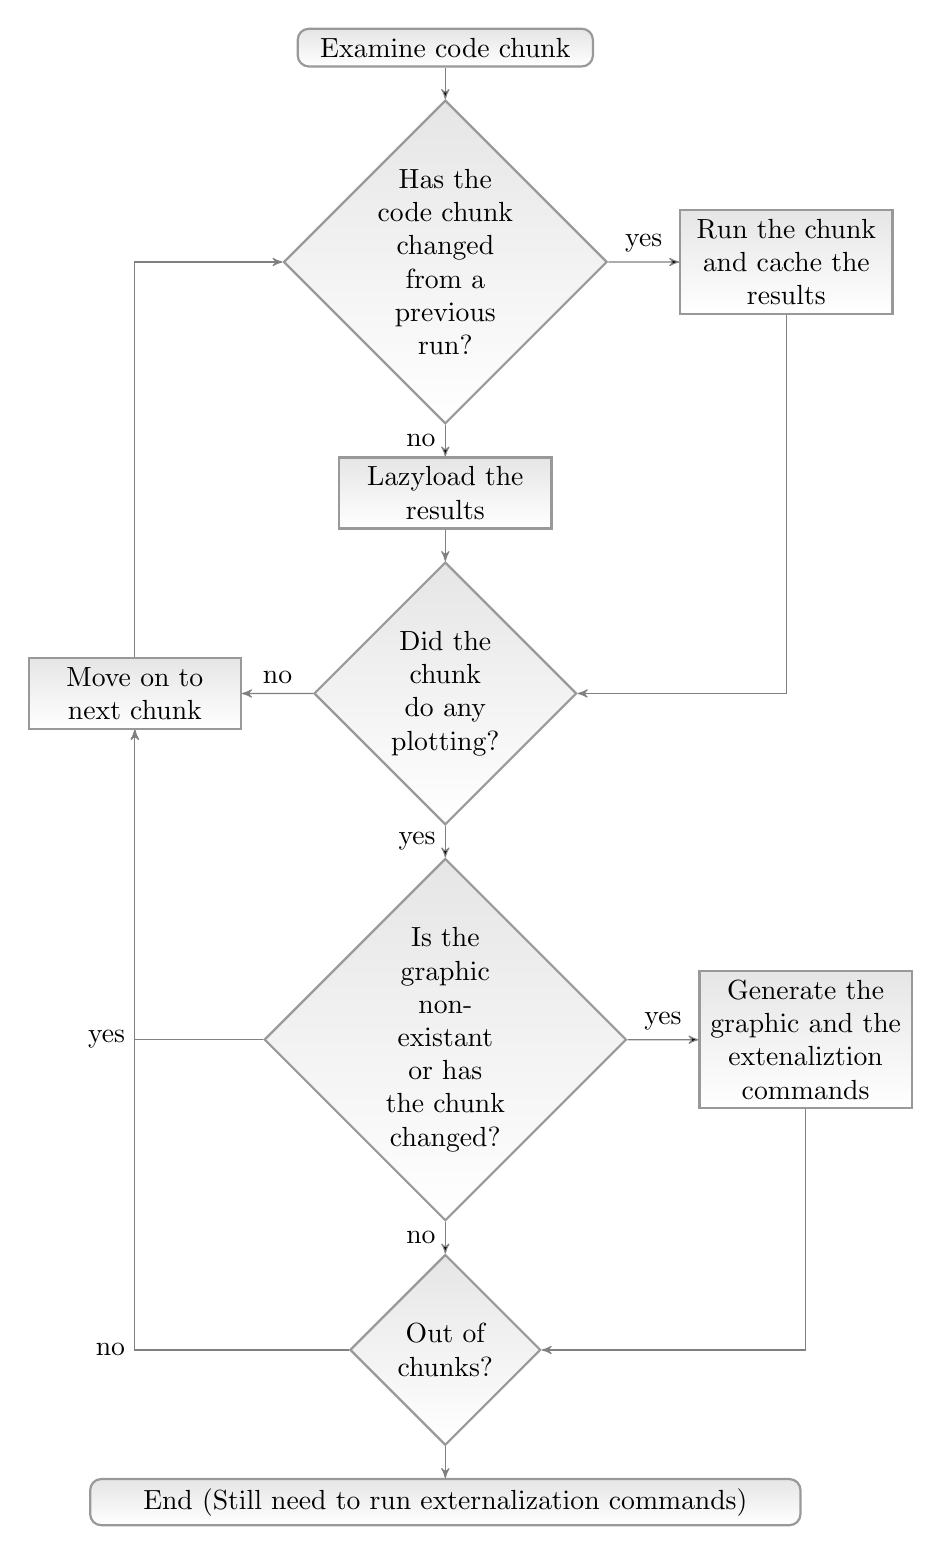
\begin{tikzpicture}
    [
    node distance=4mm and 9mm,
    scale=.8,
    block/.style ={
        rectangle, 
        draw=gray!80, 
        thick, 
        top color=gray!20, 
        bottom color=white,
        text badly centered, 
        text width=7em
    },
    decision/.style={
        diamond, 
        draw=gray!80, 
        thick, 
        top color=gray!20, 
        bottom color=white,
	    text width=5em, 
	    text centered, 
	    inner sep=0pt
	},
	a/.style={
		-stealth',
		draw=gray
	}
    ]

    \node (init)[block,text width=10em,rounded corners,] {Examine code chunk};
    \node (past) [decision,below=of init] {Has the code chunk changed from a previous run?};
    \node (run) [block,right=of past] {Run the chunk and cache the results};
    \node (lazy) [block,below=of past] {Lazyload the results};
    \node (plotting) [decision,below=of lazy] {Did the chunk do any plotting?};
    \node (move) [block,left=of plotting] {Move on to next chunk};
    \node (extern)[decision,below=of plotting] {Is the graphic non-existant or has the chunk changed?};
    \node (doextern)[block,right=of extern] {Generate the graphic and the extenaliztion commands};
    \node (out)[decision,below=of extern] {Out of chunks?};
    \node (end)[block,text width=25em,rounded corners,below=of out] {End (Still need to run externalization commands)};
    
    \draw[a] (init) edge (past);
    \draw[a] (past) edge node [above] {yes} (run);
    \draw[a] (past) edge node [left] {no} (lazy);
    \draw[a] (lazy) -- (plotting);
    \draw[a] (run) |- (plotting);
    \draw[a] (plotting) edge node [left] {yes} (extern);
    \draw[a] (plotting) -- node [above] {no} (move);
    \draw[a] (extern) edge node [above] {yes} (doextern);
    \draw[a] (extern) -| node [left] {yes} (move);
    \draw[a] (extern) edge node [left] {no} (out);
    \draw[a] (out) -| node [left] {no} (move);
    \draw[a] (doextern) |- (out);
    \draw[a] (out) -- (end);
    \draw[a] (move) |- (past);
    
\end{tikzpicture}
\caption{Flow chart of modeling procedure.}\label{flow}
\end{figure}

%%%%%%%%%%%%%%%%%%%%%%%%%%%%%%%%%%%%%%%%%%%%%%%%
%%%%%%%%%%%%%%%%%%%%%%%%%%%%%%%%%%%%%%%%%%%%%%%%
\section{Consistency in style between graphics and text}
%% initial calculations


 In Figure \ref{normalSweave}, notice the inconsistency in font and size between the default \lang{R} output and the default \LaTeX{} output.  Fonts and font sizes can be changed from \lang{R} but it is hard to be precise.  What if you decide to change the font and and point size of your entire document?  In Figure \ref{pgfSweave-hist} and \ref{pgfSweave-tikz-hist} the text is consistent with the rest of the document.

\begin{figure}[!ht]
\begin{minipage}{.45\linewidth}
\centering

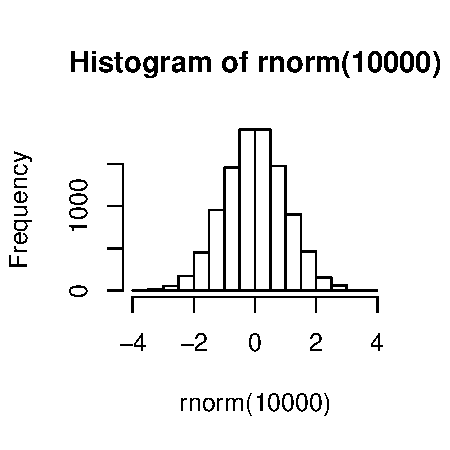
\includegraphics{figs/fig-normalSweave}
\caption{This is normal \pkg{Sweave}.}\label{normalSweave}
\end{minipage}
\begin{minipage}[!ht]{.45\linewidth}
%% pgf file will get regenerated every time slowing down the whole compilation.
%% even though cache=TRUE. 
\centering


\beginpgfgraphicnamed{figs/fig-pgfSweave-hist}
% Created by Eps2pgf 0.7.0 (build on 2008-08-24) on Fri Dec 03 11:45:25 MST 2010
\begin{pgfpicture}
\pgfpathmoveto{\pgfqpoint{0cm}{0cm}}
\pgfpathlineto{\pgfqpoint{7.62cm}{0cm}}
\pgfpathlineto{\pgfqpoint{7.62cm}{7.62cm}}
\pgfpathlineto{\pgfqpoint{0cm}{7.62cm}}
\pgfpathclose
\pgfusepath{clip}
\begin{pgfscope}
\begin{pgfscope}
\end{pgfscope}
\begin{pgfscope}
\pgfpathmoveto{\pgfqpoint{0cm}{0cm}}
\pgfpathlineto{\pgfqpoint{7.62cm}{0cm}}
\pgfpathlineto{\pgfqpoint{7.62cm}{7.62cm}}
\pgfpathlineto{\pgfqpoint{0cm}{7.62cm}}
\pgfpathclose
\pgfusepath{clip}
\begin{pgfscope}
\definecolor{eps2pgf_color}{gray}{0}\pgfsetstrokecolor{eps2pgf_color}\pgfsetfillcolor{eps2pgf_color}
\pgftext[x=4.327cm,y=6.529cm,rotate=0]{Histogram of rnorm(10000)}
\end{pgfscope}
\begin{pgfscope}
\definecolor{eps2pgf_color}{gray}{0}\pgfsetstrokecolor{eps2pgf_color}\pgfsetfillcolor{eps2pgf_color}
\pgftext[x=4.32cm,y=0.772cm,rotate=0]{rnorm(10000)}
\end{pgfscope}
\begin{pgfscope}
\definecolor{eps2pgf_color}{gray}{0}\pgfsetstrokecolor{eps2pgf_color}\pgfsetfillcolor{eps2pgf_color}
\pgftext[x=0.351cm,y=4.08cm,rotate=90]{Frequency}
\end{pgfscope}
\end{pgfscope}
\begin{pgfscope}
\pgfpathmoveto{\pgfqpoint{0cm}{0cm}}
\pgfpathlineto{\pgfqpoint{7.62cm}{0cm}}
\pgfpathlineto{\pgfqpoint{7.62cm}{7.62cm}}
\pgfpathlineto{\pgfqpoint{0cm}{7.62cm}}
\pgfpathclose
\pgfusepath{clip}
\pgfsetdash{}{0cm}
\pgfsetlinewidth{0.265mm}
\pgfsetroundcap
\pgfsetroundjoin
\definecolor{eps2pgf_color}{gray}{0}\pgfsetstrokecolor{eps2pgf_color}\pgfsetfillcolor{eps2pgf_color}
\pgfpathmoveto{\pgfqpoint{2.492cm}{2.591cm}}
\pgfpathlineto{\pgfqpoint{6.388cm}{2.591cm}}
\pgfusepath{stroke}
\pgfsetdash{}{0cm}
\pgfpathmoveto{\pgfqpoint{2.492cm}{2.591cm}}
\pgfpathlineto{\pgfqpoint{2.492cm}{2.337cm}}
\pgfusepath{stroke}
\pgfsetdash{}{0cm}
\pgfpathmoveto{\pgfqpoint{3.466cm}{2.591cm}}
\pgfpathlineto{\pgfqpoint{3.466cm}{2.337cm}}
\pgfusepath{stroke}
\pgfsetdash{}{0cm}
\pgfpathmoveto{\pgfqpoint{4.44cm}{2.591cm}}
\pgfpathlineto{\pgfqpoint{4.44cm}{2.337cm}}
\pgfusepath{stroke}
\pgfsetdash{}{0cm}
\pgfpathmoveto{\pgfqpoint{5.414cm}{2.591cm}}
\pgfpathlineto{\pgfqpoint{5.414cm}{2.337cm}}
\pgfusepath{stroke}
\pgfsetdash{}{0cm}
\pgfpathmoveto{\pgfqpoint{6.388cm}{2.591cm}}
\pgfpathlineto{\pgfqpoint{6.388cm}{2.337cm}}
\pgfusepath{stroke}
\begin{pgfscope}
\pgftext[x=2.493cm,y=1.825cm,rotate=0]{-4}
\end{pgfscope}
\begin{pgfscope}
\pgftext[x=3.464cm,y=1.825cm,rotate=0]{-2}
\end{pgfscope}
\begin{pgfscope}
\pgftext[x=4.44cm,y=1.821cm,rotate=0]{0}
\end{pgfscope}
\begin{pgfscope}
\pgftext[x=5.409cm,y=1.825cm,rotate=0]{2}
\end{pgfscope}
\begin{pgfscope}
\pgftext[x=6.386cm,y=1.825cm,rotate=0]{4}
\end{pgfscope}
\pgfsetdash{}{0cm}
\pgfpathmoveto{\pgfqpoint{2.083cm}{2.7cm}}
\pgfpathlineto{\pgfqpoint{2.083cm}{5.514cm}}
\pgfusepath{stroke}
\pgfsetdash{}{0cm}
\pgfpathmoveto{\pgfqpoint{2.083cm}{2.7cm}}
\pgfpathlineto{\pgfqpoint{1.829cm}{2.7cm}}
\pgfusepath{stroke}
\pgfsetdash{}{0cm}
\pgfpathmoveto{\pgfqpoint{2.083cm}{3.403cm}}
\pgfpathlineto{\pgfqpoint{1.829cm}{3.403cm}}
\pgfusepath{stroke}
\pgfsetdash{}{0cm}
\pgfpathmoveto{\pgfqpoint{2.083cm}{4.107cm}}
\pgfpathlineto{\pgfqpoint{1.829cm}{4.107cm}}
\pgfusepath{stroke}
\pgfsetdash{}{0cm}
\pgfpathmoveto{\pgfqpoint{2.083cm}{4.81cm}}
\pgfpathlineto{\pgfqpoint{1.829cm}{4.81cm}}
\pgfusepath{stroke}
\pgfsetdash{}{0cm}
\pgfpathmoveto{\pgfqpoint{2.083cm}{5.514cm}}
\pgfpathlineto{\pgfqpoint{1.829cm}{5.514cm}}
\pgfusepath{stroke}
\begin{pgfscope}
\pgftext[x=1.328cm,y=2.7cm,rotate=90]{0}
\end{pgfscope}
\begin{pgfscope}
\pgftext[x=1.328cm,y=4.121cm,rotate=90]{1000}
\end{pgfscope}
\begin{pgfscope}
\pgftext[x=1.328cm,y=5.512cm,rotate=90]{2000}
\end{pgfscope}
\end{pgfscope}
\begin{pgfscope}
\pgfpathmoveto{\pgfqpoint{2.083cm}{2.591cm}}
\pgfpathlineto{\pgfqpoint{6.553cm}{2.591cm}}
\pgfpathlineto{\pgfqpoint{6.553cm}{5.537cm}}
\pgfpathlineto{\pgfqpoint{2.083cm}{5.537cm}}
\pgfpathclose
\pgfusepath{clip}
\pgfsetdash{}{0cm}
\pgfsetlinewidth{0.265mm}
\pgfsetroundcap
\pgfsetroundjoin
\definecolor{eps2pgf_color}{gray}{0}\pgfsetstrokecolor{eps2pgf_color}\pgfsetfillcolor{eps2pgf_color}
\pgfpathmoveto{\pgfqpoint{2.248cm}{2.7cm}}
\pgfpathlineto{\pgfqpoint{2.248cm}{2.701cm}}
\pgfpathlineto{\pgfqpoint{2.492cm}{2.701cm}}
\pgfpathlineto{\pgfqpoint{2.492cm}{2.7cm}}
\pgfpathclose
\pgfusepath{stroke}
\pgfsetdash{}{0cm}
\pgfpathmoveto{\pgfqpoint{2.492cm}{2.7cm}}
\pgfpathlineto{\pgfqpoint{2.492cm}{2.704cm}}
\pgfpathlineto{\pgfqpoint{2.735cm}{2.704cm}}
\pgfpathlineto{\pgfqpoint{2.735cm}{2.7cm}}
\pgfpathclose
\pgfusepath{stroke}
\pgfsetdash{}{0cm}
\pgfpathmoveto{\pgfqpoint{2.735cm}{2.7cm}}
\pgfpathlineto{\pgfqpoint{2.735cm}{2.71cm}}
\pgfpathlineto{\pgfqpoint{2.979cm}{2.71cm}}
\pgfpathlineto{\pgfqpoint{2.979cm}{2.7cm}}
\pgfpathclose
\pgfusepath{stroke}
\pgfsetdash{}{0cm}
\pgfpathmoveto{\pgfqpoint{2.979cm}{2.7cm}}
\pgfpathlineto{\pgfqpoint{2.979cm}{2.749cm}}
\pgfpathlineto{\pgfqpoint{3.222cm}{2.749cm}}
\pgfpathlineto{\pgfqpoint{3.222cm}{2.7cm}}
\pgfpathclose
\pgfusepath{stroke}
\pgfsetdash{}{0cm}
\pgfpathmoveto{\pgfqpoint{3.222cm}{2.7cm}}
\pgfpathlineto{\pgfqpoint{3.222cm}{2.916cm}}
\pgfpathlineto{\pgfqpoint{3.466cm}{2.916cm}}
\pgfpathlineto{\pgfqpoint{3.466cm}{2.7cm}}
\pgfpathclose
\pgfusepath{stroke}
\pgfsetdash{}{0cm}
\pgfpathmoveto{\pgfqpoint{3.466cm}{2.7cm}}
\pgfpathlineto{\pgfqpoint{3.466cm}{3.327cm}}
\pgfpathlineto{\pgfqpoint{3.709cm}{3.327cm}}
\pgfpathlineto{\pgfqpoint{3.709cm}{2.7cm}}
\pgfpathclose
\pgfusepath{stroke}
\pgfsetdash{}{0cm}
\pgfpathmoveto{\pgfqpoint{3.709cm}{2.7cm}}
\pgfpathlineto{\pgfqpoint{3.709cm}{3.961cm}}
\pgfpathlineto{\pgfqpoint{3.953cm}{3.961cm}}
\pgfpathlineto{\pgfqpoint{3.953cm}{2.7cm}}
\pgfpathclose
\pgfusepath{stroke}
\pgfsetdash{}{0cm}
\pgfpathmoveto{\pgfqpoint{3.953cm}{2.7cm}}
\pgfpathlineto{\pgfqpoint{3.953cm}{4.847cm}}
\pgfpathlineto{\pgfqpoint{4.196cm}{4.847cm}}
\pgfpathlineto{\pgfqpoint{4.196cm}{2.7cm}}
\pgfpathclose
\pgfusepath{stroke}
\pgfsetdash{}{0cm}
\pgfpathmoveto{\pgfqpoint{4.196cm}{2.7cm}}
\pgfpathlineto{\pgfqpoint{4.196cm}{5.359cm}}
\pgfpathlineto{\pgfqpoint{4.44cm}{5.359cm}}
\pgfpathlineto{\pgfqpoint{4.44cm}{2.7cm}}
\pgfpathclose
\pgfusepath{stroke}
\pgfsetdash{}{0cm}
\pgfpathmoveto{\pgfqpoint{4.44cm}{2.7cm}}
\pgfpathlineto{\pgfqpoint{4.44cm}{5.428cm}}
\pgfpathlineto{\pgfqpoint{4.683cm}{5.428cm}}
\pgfpathlineto{\pgfqpoint{4.683cm}{2.7cm}}
\pgfpathclose
\pgfusepath{stroke}
\pgfsetdash{}{0cm}
\pgfpathmoveto{\pgfqpoint{4.683cm}{2.7cm}}
\pgfpathlineto{\pgfqpoint{4.683cm}{4.893cm}}
\pgfpathlineto{\pgfqpoint{4.927cm}{4.893cm}}
\pgfpathlineto{\pgfqpoint{4.927cm}{2.7cm}}
\pgfpathclose
\pgfusepath{stroke}
\pgfsetdash{}{0cm}
\pgfpathmoveto{\pgfqpoint{4.927cm}{2.7cm}}
\pgfpathlineto{\pgfqpoint{4.927cm}{3.918cm}}
\pgfpathlineto{\pgfqpoint{5.17cm}{3.918cm}}
\pgfpathlineto{\pgfqpoint{5.17cm}{2.7cm}}
\pgfpathclose
\pgfusepath{stroke}
\pgfsetdash{}{0cm}
\pgfpathmoveto{\pgfqpoint{5.17cm}{2.7cm}}
\pgfpathlineto{\pgfqpoint{5.17cm}{3.299cm}}
\pgfpathlineto{\pgfqpoint{5.414cm}{3.299cm}}
\pgfpathlineto{\pgfqpoint{5.414cm}{2.7cm}}
\pgfpathclose
\pgfusepath{stroke}
\pgfsetdash{}{0cm}
\pgfpathmoveto{\pgfqpoint{5.414cm}{2.7cm}}
\pgfpathlineto{\pgfqpoint{5.414cm}{2.938cm}}
\pgfpathlineto{\pgfqpoint{5.657cm}{2.938cm}}
\pgfpathlineto{\pgfqpoint{5.657cm}{2.7cm}}
\pgfpathclose
\pgfusepath{stroke}
\pgfsetdash{}{0cm}
\pgfpathmoveto{\pgfqpoint{5.657cm}{2.7cm}}
\pgfpathlineto{\pgfqpoint{5.657cm}{2.793cm}}
\pgfpathlineto{\pgfqpoint{5.901cm}{2.793cm}}
\pgfpathlineto{\pgfqpoint{5.901cm}{2.7cm}}
\pgfpathclose
\pgfusepath{stroke}
\pgfsetdash{}{0cm}
\pgfpathmoveto{\pgfqpoint{5.901cm}{2.7cm}}
\pgfpathlineto{\pgfqpoint{5.901cm}{2.721cm}}
\pgfpathlineto{\pgfqpoint{6.144cm}{2.721cm}}
\pgfpathlineto{\pgfqpoint{6.144cm}{2.7cm}}
\pgfpathclose
\pgfusepath{stroke}
\pgfsetdash{}{0cm}
\pgfpathmoveto{\pgfqpoint{6.144cm}{2.7cm}}
\pgfpathlineto{\pgfqpoint{6.144cm}{2.703cm}}
\pgfpathlineto{\pgfqpoint{6.387cm}{2.703cm}}
\pgfpathlineto{\pgfqpoint{6.387cm}{2.7cm}}
\pgfpathclose
\pgfusepath{stroke}
\end{pgfscope}
\end{pgfscope}
\end{pgfpicture}

\endpgfgraphicnamed
\caption{This is from \pkg{pgfSweave} with the \code{pgf} option.}\label{pgfSweave-hist}
\end{minipage}
\end{figure}

\begin{figure}[!ht]
%% pgf file will get regenerated every time slowing down the whole compilation.
%% even though cache=TRUE. 
\centering


\beginpgfgraphicnamed{figs/fig-pgfSweave-tikz-hist}
% Created by tikzDevice version 0.5.3 on 2011-04-05 16:31:38
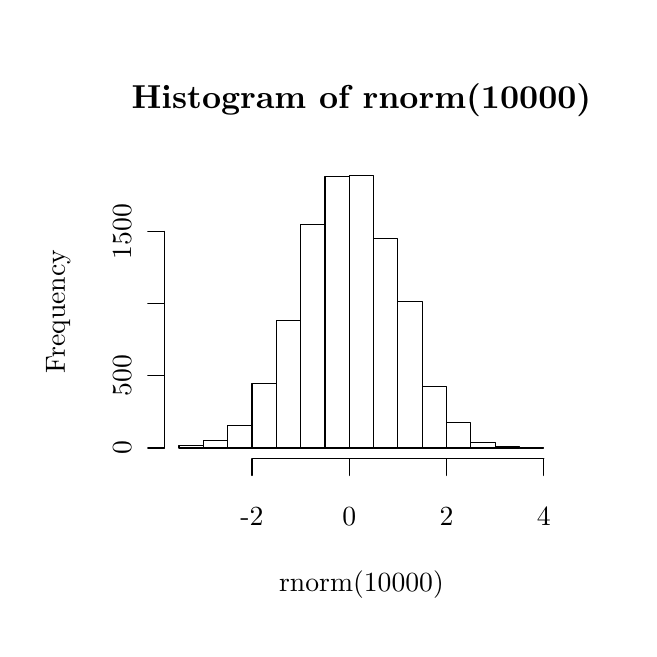
\begin{tikzpicture}[x=1pt,y=1pt]
\draw[color=white,opacity=0] (0,0) rectangle (216.81,216.81);
\begin{scope}
\path[clip] (  0.00,  0.00) rectangle (216.81,216.81);
\definecolor[named]{drawColor}{rgb}{0.40,0.41,0.40}
\definecolor[named]{drawColor}{rgb}{0.00,0.00,0.00}

\node[color=drawColor,anchor=base,inner sep=0pt, outer sep=0pt, scale=  1.20] at (120.41,187.70) {\bfseries Histogram of rnorm(10000)%
};

\node[color=drawColor,anchor=base,inner sep=0pt, outer sep=0pt, scale=  1.00] at (120.41, 13.20) {rnorm(10000)%
};

\node[rotate= 90.00,color=drawColor,anchor=base,inner sep=0pt, outer sep=0pt, scale=  1.00] at ( 13.20,114.41) {Frequency%
};
\end{scope}
\begin{scope}
\path[clip] (  0.00,  0.00) rectangle (216.81,216.81);
\definecolor[named]{drawColor}{rgb}{0.40,0.41,0.40}
\definecolor[named]{drawColor}{rgb}{0.00,0.00,0.00}

\draw[color=drawColor,line cap=round,line join=round,fill opacity=0.00,] ( 80.85, 61.20) -- (186.34, 61.20);

\draw[color=drawColor,line cap=round,line join=round,fill opacity=0.00,] ( 80.85, 61.20) -- ( 80.85, 55.20);

\draw[color=drawColor,line cap=round,line join=round,fill opacity=0.00,] (116.01, 61.20) -- (116.01, 55.20);

\draw[color=drawColor,line cap=round,line join=round,fill opacity=0.00,] (151.17, 61.20) -- (151.17, 55.20);

\draw[color=drawColor,line cap=round,line join=round,fill opacity=0.00,] (186.34, 61.20) -- (186.34, 55.20);

\node[color=drawColor,anchor=base,inner sep=0pt, outer sep=0pt, scale=  1.00] at ( 80.85, 37.20) {-2%
};

\node[color=drawColor,anchor=base,inner sep=0pt, outer sep=0pt, scale=  1.00] at (116.01, 37.20) {0%
};

\node[color=drawColor,anchor=base,inner sep=0pt, outer sep=0pt, scale=  1.00] at (151.17, 37.20) {2%
};

\node[color=drawColor,anchor=base,inner sep=0pt, outer sep=0pt, scale=  1.00] at (186.34, 37.20) {4%
};

\draw[color=drawColor,line cap=round,line join=round,fill opacity=0.00,] ( 49.20, 65.14) -- ( 49.20,143.34);

\draw[color=drawColor,line cap=round,line join=round,fill opacity=0.00,] ( 49.20, 65.14) -- ( 43.20, 65.14);

\draw[color=drawColor,line cap=round,line join=round,fill opacity=0.00,] ( 49.20, 91.21) -- ( 43.20, 91.21);

\draw[color=drawColor,line cap=round,line join=round,fill opacity=0.00,] ( 49.20,117.27) -- ( 43.20,117.27);

\draw[color=drawColor,line cap=round,line join=round,fill opacity=0.00,] ( 49.20,143.34) -- ( 43.20,143.34);

\node[rotate= 90.00,color=drawColor,anchor=base,inner sep=0pt, outer sep=0pt, scale=  1.00] at ( 37.20, 65.14) {0%
};

\node[rotate= 90.00,color=drawColor,anchor=base,inner sep=0pt, outer sep=0pt, scale=  1.00] at ( 37.20, 91.21) {500%
};

\node[rotate= 90.00,color=drawColor,anchor=base,inner sep=0pt, outer sep=0pt, scale=  1.00] at ( 37.20,143.34) {1500%
};
\end{scope}
\begin{scope}
\path[clip] ( 49.20, 61.20) rectangle (191.61,167.61);
\definecolor[named]{drawColor}{rgb}{0.40,0.41,0.40}
\definecolor[named]{drawColor}{rgb}{0.00,0.00,0.00}

\draw[color=drawColor,line cap=round,line join=round,fill opacity=0.00,] ( 54.47, 65.14) rectangle ( 63.27, 65.87);

\draw[color=drawColor,line cap=round,line join=round,fill opacity=0.00,] ( 63.27, 65.14) rectangle ( 72.06, 67.80);

\draw[color=drawColor,line cap=round,line join=round,fill opacity=0.00,] ( 72.06, 65.14) rectangle ( 80.85, 73.38);

\draw[color=drawColor,line cap=round,line join=round,fill opacity=0.00,] ( 80.85, 65.14) rectangle ( 89.64, 88.44);

\draw[color=drawColor,line cap=round,line join=round,fill opacity=0.00,] ( 89.64, 65.14) rectangle ( 98.43,111.23);

\draw[color=drawColor,line cap=round,line join=round,fill opacity=0.00,] ( 98.43, 65.14) rectangle (107.22,145.94);

\draw[color=drawColor,line cap=round,line join=round,fill opacity=0.00,] (107.22, 65.14) rectangle (116.01,163.20);

\draw[color=drawColor,line cap=round,line join=round,fill opacity=0.00,] (116.01, 65.14) rectangle (124.80,163.67);

\draw[color=drawColor,line cap=round,line join=round,fill opacity=0.00,] (124.80, 65.14) rectangle (133.59,140.73);

\draw[color=drawColor,line cap=round,line join=round,fill opacity=0.00,] (133.59, 65.14) rectangle (142.38,118.21);

\draw[color=drawColor,line cap=round,line join=round,fill opacity=0.00,] (142.38, 65.14) rectangle (151.17, 87.45);

\draw[color=drawColor,line cap=round,line join=round,fill opacity=0.00,] (151.17, 65.14) rectangle (159.96, 74.47);

\draw[color=drawColor,line cap=round,line join=round,fill opacity=0.00,] (159.96, 65.14) rectangle (168.75, 67.23);

\draw[color=drawColor,line cap=round,line join=round,fill opacity=0.00,] (168.75, 65.14) rectangle (177.54, 65.56);

\draw[color=drawColor,line cap=round,line join=round,fill opacity=0.00,] (177.54, 65.14) rectangle (186.34, 65.25);
\end{scope}
\end{tikzpicture}

\endpgfgraphicnamed
\caption{This is from \pkg{pgfSweave} with the \code{tikz} option.}\label{pgfSweave-tikz-hist}
\end{figure}


%%%%%%%%%%%%%%%%%%%%%%%%%%%%%%%%%%%%%%%%%%%%%%%%
%%%%%%%%%%%%%%%%%%%%%%%%%%%%%%%%%%%%%%%%%%%%%%%%
\section{Sweave graphic width defaults}

The default in \code{Sweave.sty} is to fix the width of every image to 80\% of the text width by using \verb"\setkeys{Gin}{width=.8\textwidth}".  Say you have a 7 in text width and code chunk where you set \code{width=4}.  The original 4 inch wide graphic will have text size matching your document but when it is included in your document it will be scaled up to 7 inched wide and the text will get bigger!  This default is quite contrary to the philosophy of \pkg{pgfSweave}.  There are two ways around this before each code chunk you can set \verb"\setkeys{Gin}{width=<graphic width>}". Alternatively (and the recommended way) you can turn off this feature globally by using \verb"\usepackage[nogin]{Sweave}", that way the width and height of the figure are controlled by the arguments to the code chunk. 

%%%%%%%%%%%%%%%%%%%%%%%%%%%%%%%%%%%%%%%%%%%%%%%%
%%%%%%%%%%%%%%%%%%%%%%%%%%%%%%%%%%%%%%%%%%%%%%%%
\section{Command line interface\label{commandline}}

In recent versions, \pkg{pgfSweave} got an \code{R CMD} command line interface.  On Unix alikes (including Mac OS X) a symbolic link \code{\$R\_HOME/bin/pgfsweave} to \code{\$R\_HOME/library/pgfSweave/exec/pgfsweave-script.R}.  On Windows a copy of the script is made instead.  {\color{red} This script is only installed if pgfSweave is installed from source}.

Here is a listing from \code{R CMD pgfsweave --help}:

\begin{Verbatim}[frame=single]
Usage: R CMD pgfsweave [options] file

A simple front-end for pgfSweave()

The options below reference the following steps 
  (1) Run Sweave using pgfSweaveDriver
  (2) Run the pgf externalization commands
  (3) Compile the resulting tex file using texi2dvi()

Default behavior (no options) is to do (1), (2) then (3) in that order.

Options:
  -h, --help                print short help message and exit
  -v, --version             print version info and exit
  -d, --dvi                 dont use texi2dvi() option pdf=T i.e. call plain 
                            latex (defalt is pdflatex)
  -n, --graphics-only       dont do (3), do (1) then (2); ignored if 
                            --pgfsweave-only is used
  -s, --pgfsweave-only      dont do (2) or (3), only do (1)

Package repositories: 
http://github.com/cameronbracken/pgfSweave (cutting edge development)
http://r-forge.r-project.org/projects/pgfsweave/ (for precompiled packages)
\end{Verbatim}

\clearpage
%%%%%%%%%%%%%%%%%%%%%%%%%%%%%%%%%%%%%%%%%%%%%%%%
%%%%%%%%%%%%%%%%%%%%%%%%%%%%%%%%%%%%%%%%%%%%%%%%
\section{Frequently Asked Questions}

%--------------------------------------
%--------------------------------------
\ques{Can \pkg{pgfSweave} be run from the command line?}

Yes! See section \ref{commandline}.
\begin{Verbatim}
$ R CMD pgfsweave <yourfile>.Rnw
\end{Verbatim}

%--------------------------------------
%--------------------------------------
\ques{The changes to my code chunk are not being recognized.}

Occasionally \pkg{pgfSweave} suffers from overzealous caching.  In these cases it may be necessary to manually delete the cache or the figure files. This is something we need to improve but this is better than compiling too often which is what used to happen. 

%--------------------------------------
%--------------------------------------
\ques{How do I set subdirectories for figures and caches?}

This is straight out of the \pkg{Sweave} and \pkg{cacheSweave} manuals (nothing new here).  For a figures subdirectory \footnote{make sure to create the directory first!} use the \code{prefix.string} option:

\begin{verbatim}\SweaveOpts{prefix.string=figs/fig}\end{verbatim}

For a caching subdirectory use a code chunk at the beginning or your document like:
\begin{verbatim}
	<<setup,echo=F>>=
	setCacheDir("cache")
	@
\end{verbatim}

%--------------------------------------
%--------------------------------------
\ques{Why are the width and height options being ignored?}

This is another one from \pkg{Sweave}. You must use the \code{nogin} option in \code{Sweave.sty} for the width and height parameters to actually affect the size of the image in the document:
\begin{verbatim}\usepackage[nogin]{Sweave}\end{verbatim}

%--------------------------------------
%--------------------------------------
\ques{\LaTeX{}/PDF\LaTeX{} is not found in R.app (Mac OS X) and [Possibly] R.exe (Windows)}

Your latex program is not in the default search path.  Put a line such as:

\begin{verbatim}Sys.setenv("PATH" = paste(Sys.getenv("PATH"),"/usr/texbin",sep=":"))\end{verbatim}
in your \verb".Rprofile" file.  

%--------------------------------------
%--------------------------------------
\ques{I get a bunch of ``Incompatible list can't be unboxed'' errors when compiling.}

This is a problem with the CVS version of PGF.  The workaround is to load the \pkg{atbegshi} package before PGF or TikZ:

\begin{verbatim}
\usepackage{atbegshi}
\usepackage{pgf}
\end{verbatim}

or

\begin{verbatim}
\usepackage{atbegshi}
\usepackage{tikz}
\end{verbatim}

%--------------------------------------
%--------------------------------------
\ques{The vignette in \texttt{/inst/doc/} does not contain any code chunks!}

That is because the vignette in \texttt{/inst/doc/} is a ``fake'' vignette generated from the ``real'' vignette in \texttt{/inst/misc/vignette-src/}.  The reason for this extra step is  that package vignettes must be able to be compiled with \texttt{R CMD Sweave}, which is precisely what we don't want to use!

To compile the vignette yourself, download the package source, unpack it and then do the following:

\begin{verbatim}
git clone git://github.com/cameronbracken/pgfSweave.git
R CMD INSTALL pgfSweave
cd pgfSweave/inst/misc/vignette-src/
make
\end{verbatim}
Which will create \code{pgfSweave-vignette-source.pdf}


\end{document}
